
\chapter{Introduction}\label{sec:introduction}

Turbomachines are devices that transfer energy either to or from a continuously fluid by dynamic action of moving blades. While a turbine transfers energy from a fluid to a rotor, a compressor transfers energy from a rotor to a fluid. Due to a change of pressure and velocity provoked by rotating blades the enthalpy of the fluid changes, which implies a positive or negative amount of work. In a fan $(W < 0)$ the fluid pressure is increased and therefore work is needed. In contrary turbines are expanding the fluid $(\Delta p < 0)$ and result in a power-producing machine. Turbomachines are widely used and of extraordinary importance for most energy conversion processes.

\begin{figure}[H]
\centering
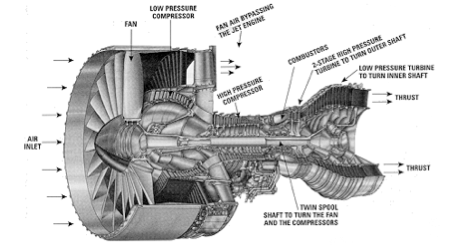
\includegraphics[width=0.7\textwidth]{pics/f1.png}
\caption{Typical Axial Flow Compressor Engine}
\label{fig:f1}
\end{figure}

